% Analítica Predictiva y Prescriptiva · TIC-60286 · Semana 5
% Árboles de clasificación
% Compilar: pdflatex week-05.tex (dos veces)
%
% Plan de los 90 minutos
%   0–5    Dónde vamos (láminas 2–3)
%   5–20   El paper: Frydman, Altman y Kao (1985), con Rudin (2019) (láminas 4–9)
%  20–65   La aplicación: el árbol de referencia, el primer corte a mano, el memorizador,
%          la poda honesta, el error sembrado, la perilla, la calibración, Barranquilla,
%          el giro de la semilla (láminas 10–19)
%  65–70   Puente: el task 5 (lámina 20)
%  70–90   Cierre: el task 4 que trajeron (lámina 21)
%
% Las cifras salen de datasets/aperturas/cifras_week05.txt y, las derivadas (el primer corte a mano,
% la calibración por hoja, el beneficio por umbral), de input/cifras_derivadas_week05.txt.
% Las figuras las genera input/_figuras_week05.R; figures/arbol_clasificacion.pdf es la figura
% base del generador del estudio (datasets/aperturas/figuras/).
% En vivo (lámina 12): el memorizador y la poda se corren en la práctica 5 (profundidad 6, mínimo 5)
% o en una sesión de R con las dos líneas de la lámina.

\documentclass{beamer}
\input{../../_beamer/preambulo_app.tex}
\semana{5}{Árboles de clasificación}

\begin{document}

%%=================================================
%% Primer slide
\begin{frame}
\titlepage
\end{frame}

%% ====================================================== 0. DÓNDE VAMOS (0–5)
\begin{frame}{Dónde vamos}
\begin{columns}[T]
\begin{column}{0.5\textwidth}
\textbf{La semana pasada:} fueron el juez. Dos consultoras, una matriz, una hoja de costos y una tabla del líder. Su veredicto (el task 4) se discute hoy, en el cierre.

\medskip
\textbf{Hoy, la pieza 5 del expediente:} su propio modelo. Un árbol de clasificación entrenado con el estudio de aperturas, leído como una política para la junta, evaluado con los mismos costos, y aplicado a los tres locales de Barranquilla.
\end{column}
\begin{column}{0.5\textwidth}
\begin{block}{La sesión}
\begin{enumerate}
  \item El paper: el primer árbol que predijo quiebras (1985).
  \item El árbol de Latitud, leído en voz alta y verificado a mano.
  \item El memorizador, la poda y un error sembrado.
  \item La perilla del umbral y los tres locales.
  \item Cierre: el task 4.
\end{enumerate}
\end{block}
\end{column}
\end{columns}
\end{frame}

\begin{frame}{Antes de empezar}
\parada{chat}{Si tuvieras que hacer \textbf{una sola pregunta} sobre un local para saber si el punto de venta sobrevive tres años, ¿cuál sería? Una línea. Leemos cinco y luego las comparamos con la pregunta que hace el árbol.}
\medskip
\small Lo que cada uno escribió es su raíz. El árbol elige la suya midiendo qué corte separa mejor a los que cerraron de los que no, entre 360 puntos de venta.
\end{frame}

\seccion{El paper: el primer árbol que predijo quiebras}
%% ====================================================== 1. EL PAPER (5–20)
\begin{frame}{Predecir la quiebra con un árbol}{Frydman, Altman y Kao (1985), \emph{Journal of Finance}}
\small
\begin{columns}[T]
\begin{column}{0.5\textwidth}
\textbf{Qué investigaron.} Si un árbol de clasificación (\emph{recursive partitioning}) predice la quiebra de empresas mejor que el método estándar de la época: el análisis discriminante del Z-score de Altman.

\medskip
\textbf{El contexto.} Un banco, un proveedor o un auditor necesitan saber qué empresas van a entrar en dificultades. La herramienta estándar era una combinación lineal de razones financieras con un punto de corte: funcionaba, pero no se leía como una regla.
\end{column}
\begin{column}{0.5\textwidth}
\textbf{Qué datos y cómo.}
\begin{itemize}\itemsep3pt
  \item Doscientas empresas, \textbf{58 quebradas}.
  \item \textbf{Veinte razones financieras} conocidas antes de la quiebra.
  \item Árboles que ensayan todos los cortes, con \textbf{costos de error asimétricos}: equivocarse con una empresa que quiebra cuesta más que con una sana.
  \item Comparados con el análisis discriminante en los mismos datos y en muestras reservadas.
\end{itemize}
\end{column}
\end{columns}
\end{frame}

\begin{frame}{Qué encontraron}
\small
\begin{itemize}\itemsep5pt
  \item El árbol \textbf{compite o gana} frente al análisis discriminante, dentro y fuera de la muestra con la que se construyó.
  \item Usa \textbf{pocas razones}: unas cuantas preguntas en secuencia (flujo de caja frente a deuda, utilidades retenidas frente a activos) bastan.
  \item Produce \textbf{reglas que un analista lee}: ``si esta razón está por debajo de tal valor y aquella por debajo de tal otro, la empresa va a quiebra''.
  \item Los \textbf{costos de cada error entran en la regla}: cambiar el costo relativo de los dos errores cambia los cortes y las hojas, no solo el punto de corte final.
\end{itemize}
\medskip
\importa{Leer el modelo completo no fue el precio de predecir peor. Y la economía de los errores no se agrega al final: está dentro del árbol.}
\end{frame}

\begin{frame}{Por qué importa para quien decide}
\begin{block}{Tres lecciones}
\begin{enumerate}\itemsep4pt
  \item Un banco necesita \textbf{una regla legible}: el comité de crédito, el regulador y el cliente rechazado tienen derecho a saber por qué.
  \item Necesita \textbf{un umbral que respete el costo} de prestarle a quien quiebra, que no es el mismo que el de negarle crédito a quien iba a pagar.
  \item Lo que importa es el desempeño \textbf{fuera de la muestra} con la que se construyó la regla; dentro de ella, cualquier árbol acierta.
\end{enumerate}
\end{block}
\parada{el puente}{Latitud tiene un estudio de 480 puntos de venta con su desenlace a tres años, doce variables de antes de abrir y tres locales en Barranquilla. Le pasa lo que a los bancos con las empresas: necesita una regla legible, un umbral con sus costos, y saber qué pasa fuera de la muestra.}
\end{frame}

\begin{frame}{Cuarenta años después: Rudin (2019)}{\emph{Nature Machine Intelligence}}
\begin{columns}[T]
\begin{column}{0.55\textwidth}
\begin{itemize}\itemsep5pt
  \item Para decisiones de alto riesgo (crédito, justicia, salud), un modelo \textbf{interpretable} y no una caja negra explicada después.
  \item Una ``explicación'' de una caja negra es otro modelo que la imita; cuando no coincide con ella, nadie sabe cuál de los dos falló.
  \item El intercambio ``más exactitud a cambio de menos legibilidad'' es menos frecuente de lo que se cree: con datos estructurados, un modelo interpretable bien construido suele empatar.
\end{itemize}
\end{column}
\begin{column}{0.45\textwidth}
\importa{Cuando la junta pregunte ``¿por qué este local y no aquel?'', la respuesta tiene que caber en una lámina. El árbol cabe. Un bosque de quinientos árboles, no; por eso, cuando el bosque decide, el árbol habla por él: es su \textbf{vocero}.}
\end{column}
\end{columns}
\end{frame}

\seccion{La aplicación: el árbol de Latitud}
%% ====================================================== 2. LA APLICACIÓN (20–65)
\begin{frame}{El árbol de referencia, leído en voz alta}
\begin{columns}[T]
\begin{column}{0.58\textwidth}
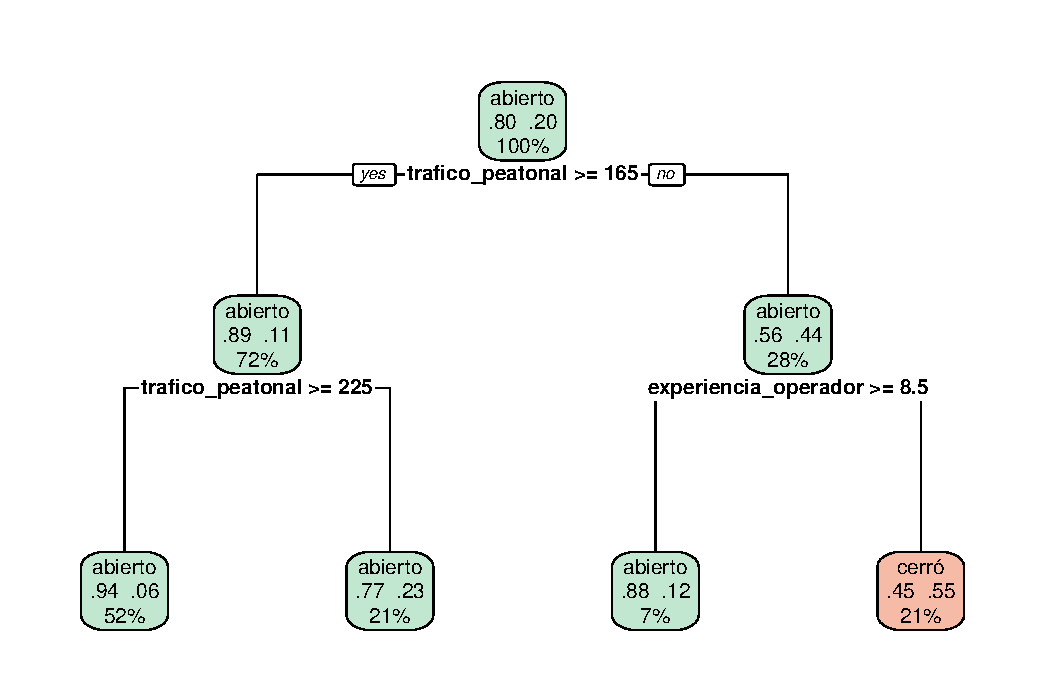
\includegraphics[width=\textwidth]{figures/arbol_clasificacion.pdf}
\end{column}
\begin{column}{0.42\textwidth}
\footnotesize
Profundidad 2, mínimo 15 por hoja, 360 puntos de venta, doce columnas de antes de abrir.
\medskip

\textbf{Tráfico de 225 o más:} cierra 1 de cada 10 (p = 0.06, n = 187).

\textbf{Tráfico entre 165 y 224:} 2 de cada 10 (0.23, n = 74).

\textbf{Tráfico bajo, operador con 9 años o más:} 1 de cada 10 (0.12, n = 24).

\textbf{Tráfico bajo, menos de 9 años:} 5 de cada 10 (0.55, n = 75). La única hoja que predice ``cierra''.
\medskip

¿Coincide la raíz con la pregunta de ustedes?
\end{column}
\end{columns}
\end{frame}

\begin{frame}{No creer, verificar: el primer corte a mano}
\begin{columns}[T]
\begin{column}{0.55\textwidth}
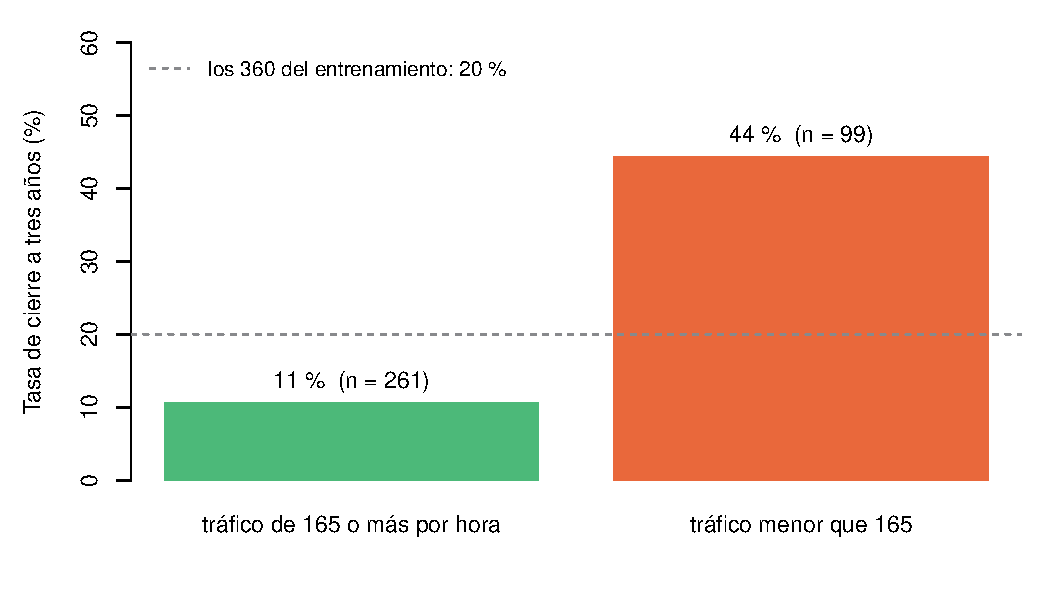
\includegraphics[width=\textwidth]{figures/primer_corte.pdf}

\medskip
{\scriptsize Desde el CSV, con los 360 de entrenamiento (\texttt{entr}):\\[2pt]
\texttt{tapply(entr\$estado\_3a == "cerró",}\\
\texttt{\ \ \ \ \ \ \ entr\$trafico\_peatonal < 164.5, mean)}}
\end{column}
\begin{column}{0.45\textwidth}
\small
El árbol dice que el mejor corte es el tráfico en 164.5. Se rehace a mano:
\medskip

\textbf{Menos de 165 por hora:} cierran 44 de cada 100 (0.444, n = 99).

\textbf{165 o más:} 11 de cada 100 (0.107, n = 261).
\medskip

\importa{Un corte del árbol es una tabla cruzada. Si no la puedes rehacer, no la puedes defender.}
\end{column}
\end{columns}
\end{frame}

\begin{frame}{El memorizador, en vivo}
\begin{columns}[T]
\begin{column}{0.55\textwidth}
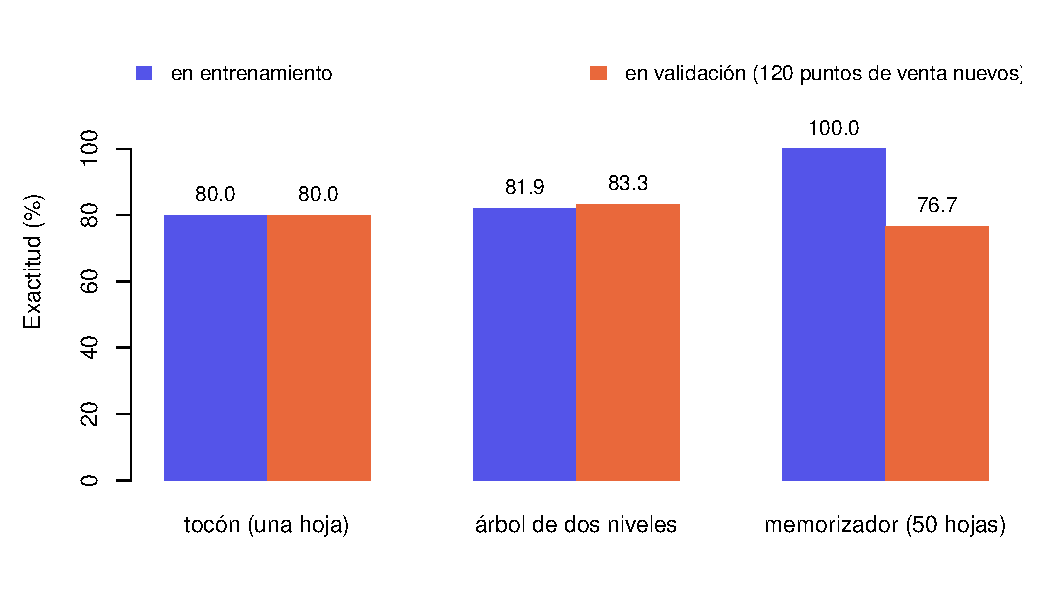
\includegraphics[width=\textwidth]{figures/memorizador.pdf}

\medskip
{\scriptsize Sin frenos: \texttt{cp = 0.0001}, \texttt{minsplit = 2}, \texttt{minbucket = 1}. En la práctica, profundidad 6 y mínimo 5 muestran lo mismo.}
\end{column}
\begin{column}{0.45\textwidth}
\small
\begin{itemize}\itemsep3pt
  \item \textbf{50 hojas.} Exactitud \textbf{1.000} en entrenamiento.
  \item En validación, \textbf{0.767}: peor que no hacer nada (0.800).
  \item El árbol de dos niveles: 0.819 y 0.833. Lo que aprendió, lo repite.
\end{itemize}
\medskip
\importa{El estudiante que se sabía el parcial de memoria. La cifra de entrenamiento no se reporta como desempeño.}
\end{column}
\end{columns}
\end{frame}

\begin{frame}{La poda honesta: la tabla cp y la regla 1-SE}
\begin{columns}[T]
\begin{column}{0.55\textwidth}
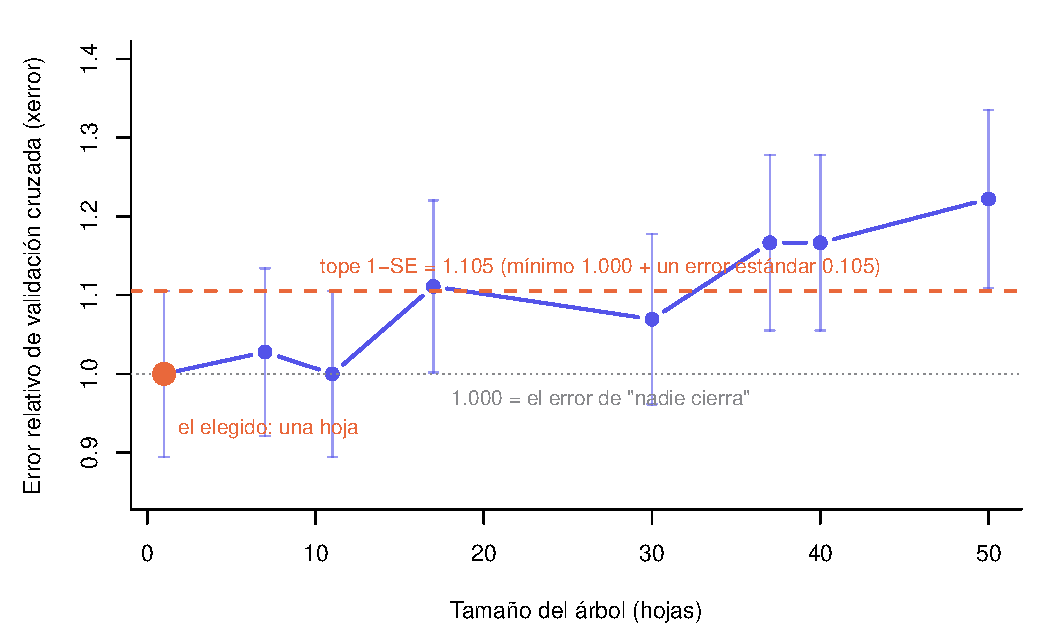
\includegraphics[width=\textwidth]{figures/tabla_cp.pdf}
\end{column}
\begin{column}{0.45\textwidth}
\small
\texttt{rpart} corre validación cruzada mientras entrena: para cada tamaño, el error relativo a ``nadie cierra'' (1.000).
\smallskip

\textbf{Regla 1-SE:} mínimo (1.000) más un error estándar (0.105) = tope \textbf{1.105}. El árbol más simple bajo el tope tiene \textbf{una hoja}: el tocón.
\smallskip

\textbf{¿Falló algo?} No. Con dos de cada diez cerrados, ningún corte le gana a ``nadie cierra'' en exactitud por más de un error estándar.
\smallskip

\textbf{¿Inútil?} En exactitud, 0.833 contra 0.800 es empate técnico ($\pm$ 0.068). En cierres encontrados, \textbf{15 de 24} contra \textbf{0}. Eso es lo que importa.
\end{column}
\end{columns}
\end{frame}

\begin{frame}{Un árbol mejor}
\begin{columns}[T]
\begin{column}{0.55\textwidth}
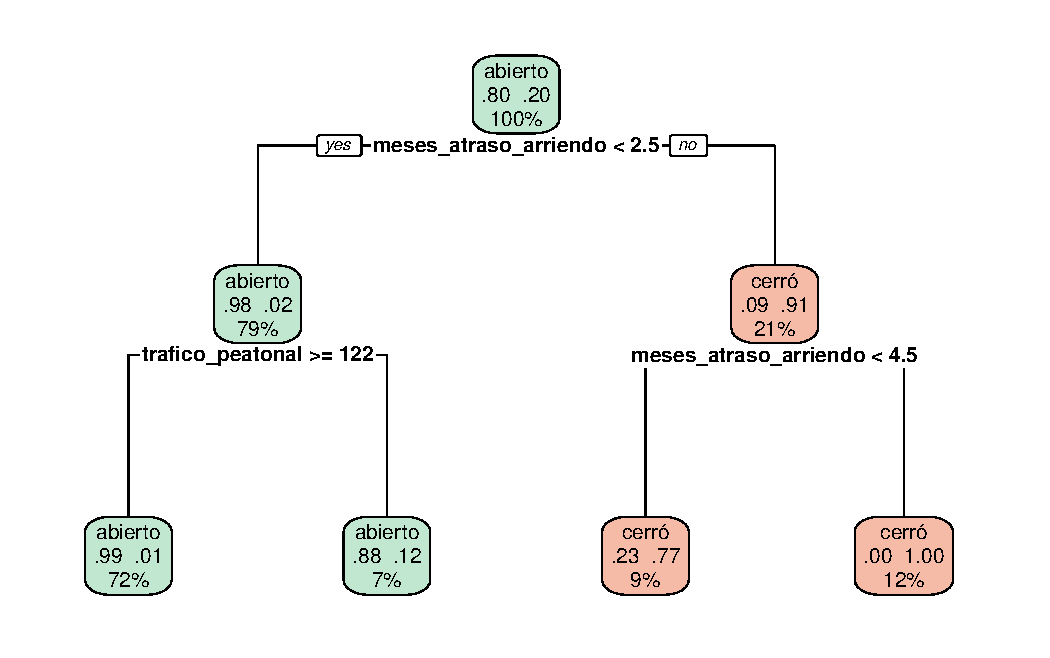
\includegraphics[width=\textwidth]{figures/arbol_fuga.pdf}
\end{column}
\begin{column}{0.45\textwidth}
\small
Un equipo entrena otro árbol con las mismas 360 filas: raíz en \texttt{meses\_atraso\_arriendo < 2.5} y \textbf{94.2\,\%} de exactitud en validación, frente a 83.3\,\%.
\medskip

\parada{error sembrado}{¿Qué está mal? Dos minutos en parejas. Pista: ¿cuántos meses de arriendo debe un local que no ha abierto?}
\medskip

\footnotesize El atraso se acumula \emph{mientras} el punto de venta cierra: predice el pasado. Para Barranquilla vale cero por definición. El salto a 0.942 es la alarma de la semana 3.
\end{column}
\end{columns}
\end{frame}

\begin{frame}{La perilla: el umbral con los costos de la semana 4}
\begin{columns}[T]
\begin{column}{0.55\textwidth}
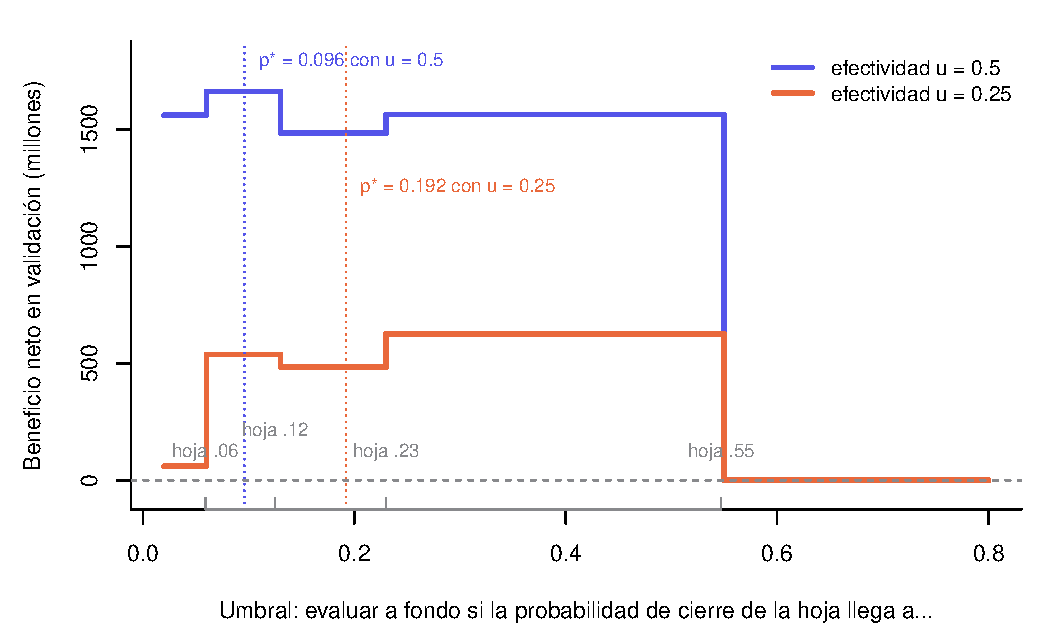
\includegraphics[width=\textwidth]{figures/umbral_beneficio.pdf}
\end{column}
\begin{column}{0.45\textwidth}
\small
La hoja no dice ``cierra'': dice 6, 12, 23 o 55 de cada 100. El 0.5 que trae el programa no es de Latitud.
\medskip

\textbf{En palabras:} evaluar a fondo cuando $p \times u \times V > c$; el umbral es $p^* = c / (u \times V)$.

\medskip
$u = 0.5$: $p^* = 12 / 125 = \mathbf{0.096}$.\\
Se evalúan tres de las cuatro hojas.

\smallskip
$u = 0.25$: $p^* = 12 / 62.5 = \mathbf{0.192}$.\\
Solo las hojas de 0.23 y 0.55.
\medskip

\textbf{Con cupo} (presupuesto para evaluar uno o dos de los tres locales), el umbral deja de importar: se ordena por riesgo.
\end{column}
\end{columns}
\end{frame}

\begin{frame}{¿Las probabilidades son creíbles? Calibración por tramos}
\begin{columns}[T]
\begin{column}{0.52\textwidth}
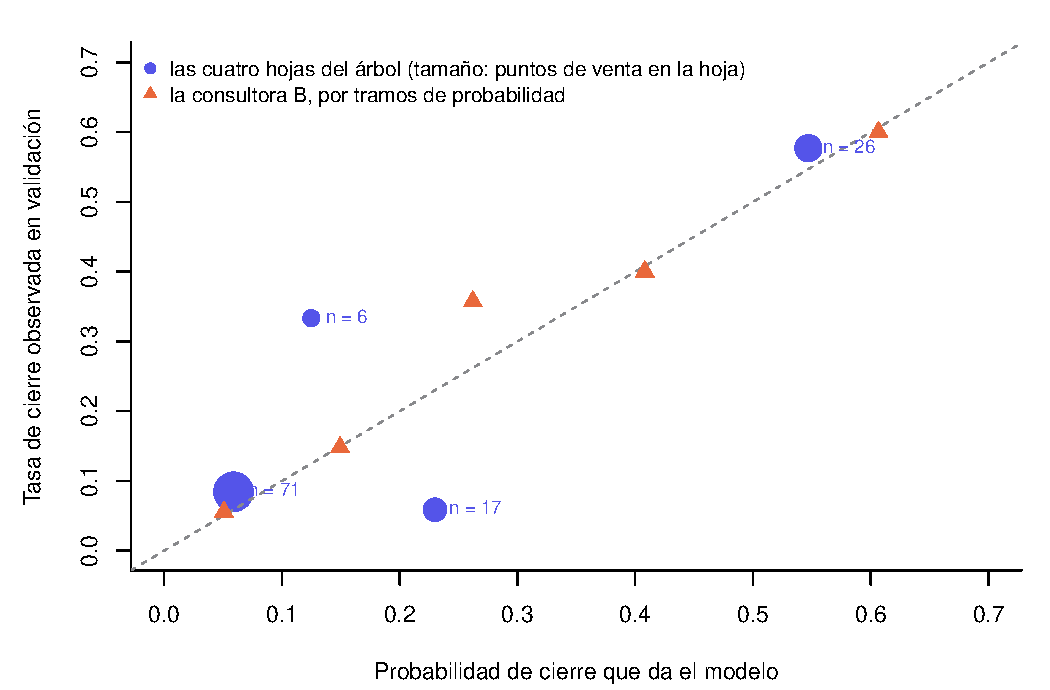
\includegraphics[width=\textwidth]{figures/calibracion.pdf}
\end{column}
\begin{column}{0.48\textwidth}
\footnotesize
Entre los puntos de venta a los que el árbol les da 55\,\%, ¿cierra cerca del 55\,\%?
\medskip

{\scriptsize
\begin{tabular}{@{}lrr@{}}
\toprule
Hoja del árbol & Observada & n \\
\midrule
p = 0.06 & 0.085 & 71 \\
p = 0.12 & 0.333 & 6 \\
p = 0.23 & 0.059 & 17 \\
p = 0.55 & 0.577 & 26 \\
\midrule
B, tramo 0 a 0.1 & 0.056 & 54 \\
B, 0.1 a 0.2 & 0.148 & 27 \\
B, 0.2 a 0.3 & 0.357 & 14 \\
B, 0.3 a 0.5 & 0.400 & 15 \\
B, 0.5 a 1 & 0.600 & 10 \\
\bottomrule
\end{tabular}}
\medskip

Las hojas grandes son creíbles; las pequeñas oscilan con uno o dos cierres. Por eso el umbral no rinde lo que $p^*$ promete: la hoja de 0.23 decepcionó.
\end{column}
\end{columns}
\end{frame}

\begin{frame}{Los tres locales de Barranquilla, con asteriscos}
\begin{columns}[T]
\begin{column}{0.55\textwidth}
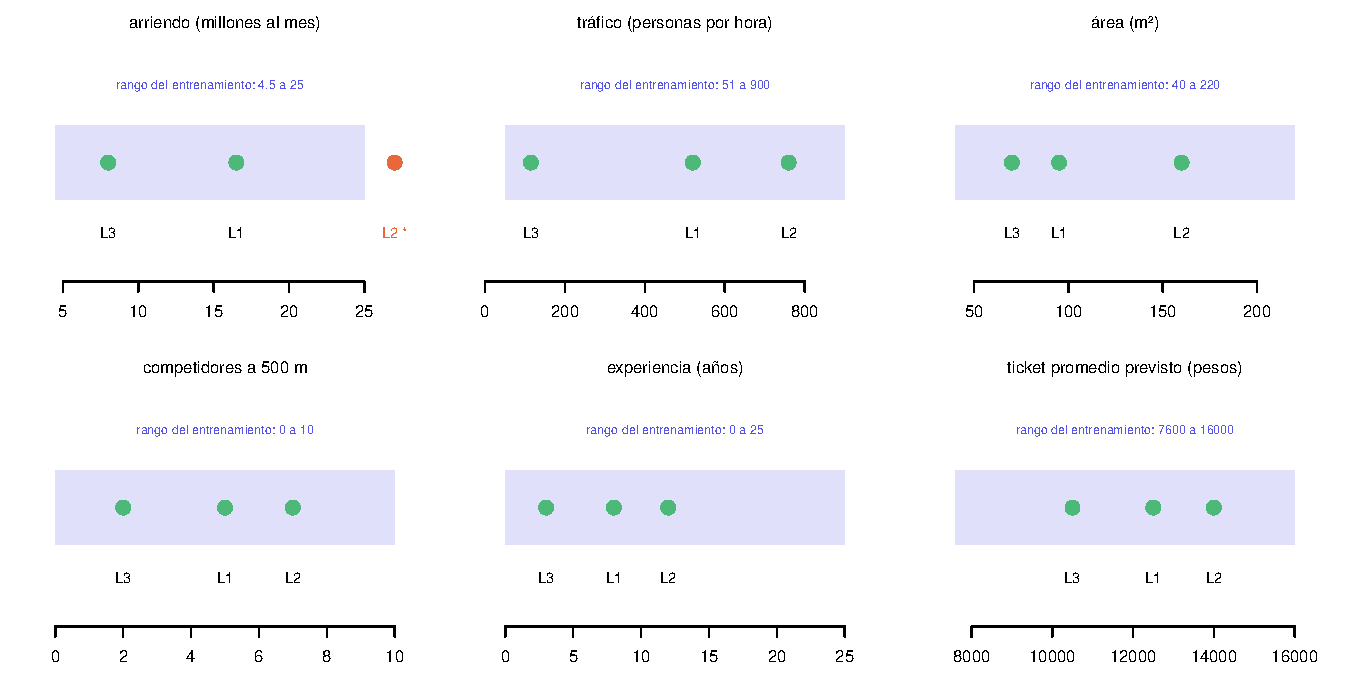
\includegraphics[width=\textwidth]{figures/locales_soporte.pdf}
\end{column}
\begin{column}{0.45\textwidth}
\footnotesize
{\scriptsize
\begin{tabular}{@{}lcl@{}}
\toprule
Local & p & Nota \\
\midrule
1 & 0.059 & * ciudad \\
2 & 0.059 & * ciudad, arriendo 27 \\
3 & 0.547 & * ciudad \\
\bottomrule
\end{tabular}}
\medskip

\textbf{Orden por riesgo:} 3, luego 1 y 2 empatados. \textbf{Con $p^* = 0.096$:} se evalúa a fondo el 3; 1 y 2 pasan.
\smallskip

\textbf{* Fuera del soporte.} Ningún punto de venta del estudio está en Barranquilla; el local 2 paga 27 millones y el máximo del entrenamiento es 25. El árbol responde igual: que responda no significa que sepa.

\importa{La nota de extrapolación va pegada a la cifra. Sin nota, no cuenta.}
\end{column}
\end{columns}
\end{frame}

\begin{frame}{El giro: otra semilla, otro segundo nivel}
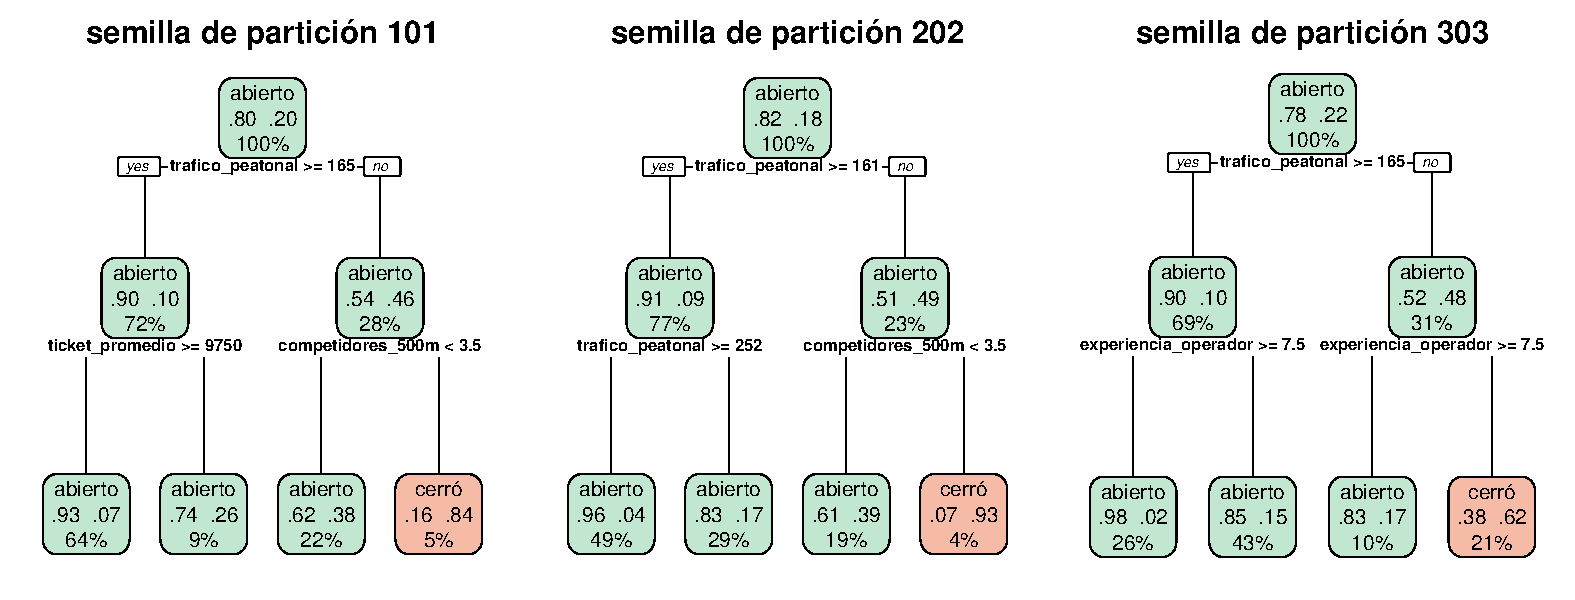
\includegraphics[width=\textwidth]{figures/estabilidad.pdf}
\begin{columns}[T]
\begin{column}{0.55\textwidth}
\small Tres particiones distintas del mismo estudio. La raíz es siempre el tráfico (164.5, 160.5 y 164.5). El segundo nivel cambia: ticket promedio y competidores; tráfico y competidores; experiencia.
\end{column}
\begin{column}{0.45\textwidth}
\parada{el giro}{¿Qué sí le decimos a la junta y qué nos guardamos? Una línea por equipo.}
\end{column}
\end{columns}
\end{frame}

\begin{frame}{Lo que importa}
\importa{%
\begin{enumerate}\itemsep5pt
  \item \textbf{El árbol es una política que se lee.} Cuatro reglas, cada una con cuántos de cada diez y con cuántos puntos de venta la respaldan. Se traduce sin decir nodo ni corte, y sin decir causa.
  \item \textbf{La cifra que vale es la de validación.} El memorizador saca 1.000 en entrenamiento y 0.767 en validación; la poda honesta deja el tocón porque la exactitud engaña con clases raras. Se reportan exactitud \emph{y} sensibilidad.
  \item \textbf{La hoja es una probabilidad y el umbral es del negocio.} $p^* = c / (u \times V)$: 0.096 o 0.192 según la efectividad. Con cupo, se ordena por riesgo.
  \item \textbf{Lo que aguanta cuando cambia la muestra es lo que se cuenta.} La raíz sí; el segundo nivel, no. Y fuera del soporte, asterisco.
\end{enumerate}}
\end{frame}

\seccion{El task y el cierre}
%% ====================================================== 3. PUENTE (65–70)
\begin{frame}{Task 5: el árbol del equipo}
\begin{columns}[T]
\begin{column}{0.55\textwidth}
\textbf{Qué se entrega} (una página, en equipo, antes de la sesión 6; se hace con la práctica 5, sin código):
\begin{itemize}\itemsep3pt
  \item tres reglas del árbol traducidas para la junta, con p y n (1.5);
  \item la tabla del líder con la fila del árbol del equipo, contra el sobre y con margen (1.5);
  \item el umbral elegido con los costos y qué locales pasan (1.0);
  \item los tres locales con su riesgo y su nota de extrapolación (0.5);
  \item el acta y la declaración (0.5).
\end{itemize}
\end{column}
\begin{column}{0.45\textwidth}
\begin{exampleblock}{En el cierre de la sesión 6}
Cada equipo traduce una rama en voz alta. Dos preguntas: ¿el árbol cambió con otra semilla y qué aguantó? ¿Qué sí se le dice a la junta?
\end{exampleblock}
\begin{alertblock}{Lo que no cuenta}
La exactitud de entrenamiento. Un árbol con \texttt{meses\_atraso\_arriendo}. Una hoja de menos de diez puntos de venta. Barranquilla sin asterisco.
\end{alertblock}
\end{column}
\end{columns}
\end{frame}

%% ====================================================== 4. CIERRE (70–90)
\begin{frame}{Cierre: el juez de modelos (task 4)}
\begin{enumerate}\itemsep6pt
  \item \textbf{Encuesta} (2 minutos): ¿quién eligió A, quién B, quién ninguna? Se cuenta a mano alzada.
  \item \textbf{Dos equipos al azar, dos minutos cada uno} (6 minutos): su tabla del líder y su recomendación. A encuentra 10 de 24 cierres con 13 evaluaciones; B, 12 con 25.
  \item \textbf{El giro de costos} (8 minutos): con efectividad 0.5 gana B (1.200 frente a 1.094 millones); con 0.25 gana A (469 frente a 450). ¿Qué costo volteó su elección? La efectividad de quiebre es 0.288; la pérdida evitada de quiebre, 144 millones.
  \item \textbf{La pregunta de hoy} (2 minutos): el árbol encuentra 15 de 24 con 26 evaluaciones. ¿Entra a la tabla como líder, como colíder o como nada? ¿Con qué cifra lo defienden?
  \item \textbf{Dudas} (2 minutos): la práctica 5 y la entrega del task 5.
\end{enumerate}
\end{frame}

\begin{frame}{Referencias}
\small
\begin{itemize}\itemsep4pt
  \item Frydman, H., Altman, E. I. y Kao, D.-L. (1985). Introducing recursive partitioning for financial classification: the case of financial distress. \emph{The Journal of Finance}, 40(1), 269--291.
  \item Rudin, C. (2019). Stop explaining black box machine learning models for high stakes decisions and use interpretable models instead. \emph{Nature Machine Intelligence}, 1(5), 206--215.
  \item Altman, E. I. (1968). Financial ratios, discriminant analysis and the prediction of corporate bankruptcy. \emph{The Journal of Finance}, 23(4), 589--609.
  \item Breiman, L., Friedman, J., Olshen, R. y Stone, C. (1984). \emph{Classification and Regression Trees}. Wadsworth.
  \item Sosa Escudero, W. (2019). \emph{Big data}. Siglo XXI. El capítulo sobre aprendizaje automático.
\end{itemize}
\end{frame}

\end{document}
